\begin{pastexam}[label={px:gw3-104-ds-02}]{關務三等資訊處理 104 年 第二題}
（申論；25 分）

在計算學生成績的程式中，按成績的高低分為五級，且用 IF 指令，其程式如下：
\begin{quote}
\small
\begin{tabbing}
\hspace*{2em}\=\hspace*{2em}\=\hspace*{2em}\=\hspace*{2em}\=\hspace*{2em}\=\kill
if S$<$60\\
\> then G = `F'\\
else if S$<$70\\
\>\> then G = `D'\\
\> else if S$<$80\\
\>\>\> then G = `C'\\
\>\> else if S$<$90\\
\>\>\>\> then G = `B'\\
\>\>\> Else G = `A'
\end{tabbing}
\end{quote}
若學生在五個等級中的分布是不平均的，分布機率如下表：
\begin{center}
\begin{tabular}{|c|c|c|c|c|c|}
\hline
分數（Score） & 90-100 & 80-89 & 70-79 & 60-69 & 0-59 \\ \hline
等第（Grade） & A & B & C & D & F \\ \hline
機率 & 0.05 & 0.30 & 0.50 & 0.1 & 0.05 \\ \hline
\end{tabular}
\end{center}
假設學生人數為 5000 人，請回答下列問題：
\begin{itemize}[leftmargin=2.2em, nosep]
\item[㈠] 請畫出 IF 指令的二元樹分析圖並分析此 IF 指令可能的比較次數。（10 分）
\item[㈡] 若用最佳化二元樹修正 IF 指令，請畫出該二元樹，並分析 IF 指令可能的比較次數。（10 分）
\item[㈢] 可使用什麼資料結構，使程式指令更為精簡，並請說明。（5 分）
\end{itemize}
\end{pastexam}

\begin{pastsoln}
答案：㈠ 每人平均 $3.15$ 次，$5000$ 人共 $15750$ 次。 ㈡ 先比 $S < 80$，每人平均 $2.15$ 次，共 $10750$ 次。
㈢ 用陣列做查表，以 $S$ 的十位數為索引，不必比較。

每個 \texttt{if} 比較一次。 判斷樹的內部節點是比較，葉子是等第；一個等第的比較次數等於它的葉子深度（根的深度
算 $1$ 層比較）。 平均比較次數是 $\sum (\text{機率} \times \text{比較次數})$。

\textbf{㈠ 原來的 IF。} 依序比 $S < 60$、$S < 70$、$S < 80$、$S < 90$，是一條往右長的鏈：
\begin{center}
\begin{tikzpicture}[c/.style={draw,rounded corners=2pt,inner sep=2pt,font=\small},
  g/.style={draw,circle,inner sep=1pt,minimum size=5.5mm,font=\small},
  level distance=10mm, sibling distance=18mm, edge from parent/.style={draw}]
\node[c] {$S < 60$}
  child {node[g] {F} edge from parent node[left,font=\scriptsize] {是}}
  child {node[c] {$S < 70$}
    child {node[g] {D} edge from parent node[left,font=\scriptsize] {是}}
    child {node[c] {$S < 80$}
      child {node[g] {C} edge from parent node[left,font=\scriptsize] {是}}
      child {node[c] {$S < 90$}
        child {node[g] {B} edge from parent node[left,font=\scriptsize] {是}}
        child {node[g] {A} edge from parent node[right,font=\scriptsize] {否}}
        edge from parent node[right,font=\scriptsize] {否}}
      edge from parent node[right,font=\scriptsize] {否}}
    edge from parent node[right,font=\scriptsize] {否}};
\end{tikzpicture}
\end{center}
比較次數：F 是 $1$ 次，D $2$ 次，C $3$ 次，B 和 A 都是 $4$ 次。 可能的比較次數是 $1 \sim 4$ 次，平均
\[
0.05 \cdot 1 + 0.1 \cdot 2 + 0.5 \cdot 3 + 0.3 \cdot 4 + 0.05 \cdot 4 = 0.05 + 0.2 + 1.5 + 1.2 + 0.2 = 3.15,
\]
$5000$ 人共約 $5000 \times 3.15 = 15750$ 次比較。 問題在最多人（$50\%$）的 C 要比 $3$ 次，$30\%$ 的 B 要比 $4$ 次。

\textbf{㈡ 最佳化二元樹。} 葉子的左右順序固定是 F、D、C、B、A（分數由低到高），要選一棵判斷樹讓
$\sum q_i \cdot \text{深度}_i$ 最小，這是只有外部節點權重的最佳二元搜尋樹（資結書第~18.4~節）。 設 $W(i,j)$ 是葉子 $i..j$
的機率和，$\mathit{cost}(i,j) = \min_k \{\mathit{cost}(i,k) + \mathit{cost}(k+1,j)\} + W(i,j)$，單一葉子的 $\mathit{cost} = 0$。
全部五個葉子的 $\mathit{cost}(1,5)$ 就是平均比較次數。 只有五個葉子，根有四種選法；
根的那一次比較每個人都要做，貢獻 $W = 1$，再加上左右兩邊各自的最佳值：
\begin{center}
\begin{tabular}{llll}
\toprule
根 & 左邊（最佳值） & 右邊（最佳值） & 平均比較次數 \\
\midrule
$S < 60$ & F（$0$） & D C B A（$1.9$） & $1 + 0 + 1.9 = 2.9$ \\
$S < 70$ & F D（$0.15$） & C B A（$1.2$） & $1 + 0.15 + 1.2 = 2.35$ \\
$S < 80$ & F D C（$0.8$） & B A（$0.35$） & $1 + 0.8 + 0.35 = \mathbf{2.15}$ \\
$S < 90$ & F D C B（$1.75$） & A（$0$） & $1 + 1.75 + 0 = 2.75$ \\
\bottomrule
\end{tabular}
\end{center}
（例如左邊 F、D：只要再比一次 $S < 60$，$\mathit{cost} = 0.05 + 0.1 = 0.15$；F D C 的最佳是先比 $S < 70$，
$\mathit{cost} = 0.65 + 0.15 = 0.8$。）
以最好的根 $S < 80$ 為例：左邊 F、D、C 再以 $S < 70$ 分開（C 只要再比 $1$ 次，F、D 再比 $S < 60$），右邊 B、A 用
$S < 90$ 分開。
\begin{center}
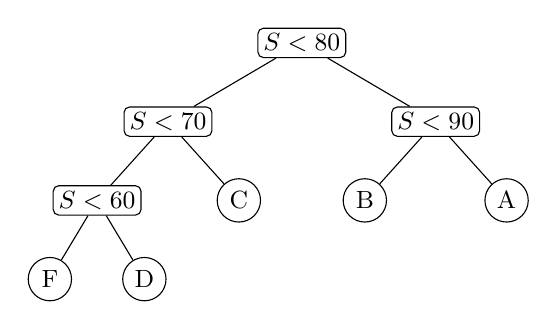
\begin{tikzpicture}[c/.style={draw,rounded corners=2pt,inner sep=2pt,font=\small},
  g/.style={draw,circle,inner sep=1pt,minimum size=5.5mm,font=\small},
  level distance=10mm, level 1/.style={sibling distance=34mm}, level 2/.style={sibling distance=18mm},
  level 3/.style={sibling distance=12mm}, edge from parent/.style={draw}]
\node[c] {$S < 80$}
  child {node[c] {$S < 70$}
    child {node[c] {$S < 60$} child {node[g] {F}} child {node[g] {D}}}
    child {node[g] {C}}}
  child {node[c] {$S < 90$} child {node[g] {B}} child {node[g] {A}}};
\end{tikzpicture}
\end{center}
（左分支是「是」，右分支是「否」。）比較次數：C、B、A 都是 $2$ 次，F、D 是 $3$ 次，可能的比較次數是 $2 \sim 3$ 次，平均
\[
0.5 \cdot 2 + 0.3 \cdot 2 + 0.05 \cdot 2 + 0.05 \cdot 3 + 0.1 \cdot 3 = 1.0 + 0.6 + 0.1 + 0.15 + 0.3 = 2.15,
\]
$5000$ 人共約 $10750$ 次，比原來少 $5000$ 次。 改寫成 IF 指令：
\begin{quote}
\small
\begin{tabbing}
\hspace*{2em}\=\hspace*{2em}\=\hspace*{2em}\=\kill
if S $<$ 80 then\\
\> if S $<$ 70 then\\
\>\> if S $<$ 60 then G = `F' else G = `D'\\
\> else G = `C'\\
else\\
\> if S $<$ 90 then G = `B' else G = `A'
\end{tabbing}
\end{quote}

\textbf{㈢ 查表。} 用一個陣列當對照表：分數 $0 \sim 100$，以十位數 $\lfloor S / 10 \rfloor$（$0 \sim 10$）為索引，
\[
\mathit{grade}[0..10] = \texttt{F F F F F F D C B A A},
\]
程式只剩一行 \texttt{G = grade[S / 10]}。 陣列可以用索引在 $O(1)$ 時間直接存取（資結書第~4.1~節），完全不用比較，
程式也不必隨等第數變長；要改分級標準時只改表格內容。 （也可以對 $\lfloor S/10 \rfloor$ 用 \texttt{switch}／\texttt{case}，
但查表最精簡。）
\end{pastsoln}
